% FEA Membranes - Verification & Validation Record
% Compile with pdfLaTeX (Overleaf default compiler works as-is).
\documentclass[11pt,a4paper]{article}

\usepackage[margin=2.2cm]{geometry}
\usepackage{booktabs}
\usepackage{amsmath}
\usepackage{tikz}
\usetikzlibrary{arrows.meta,patterns,decorations.pathmorphing,decorations.markings,calc}
\usepackage{caption}
\usepackage{float}
\usepackage[colorlinks=true,linkcolor=blue!50!black,urlcolor=blue!50!black]{hyperref}
\usepackage{parskip}

\captionsetup{font=small,labelfont=bf}

% ---------- TikZ styles shared by all case sketches ----------
\tikzset{
  fnode/.style={circle,fill=black,inner sep=1.2pt},          % FE node
  mnode/.style={circle,draw=black,fill=white,inner sep=1.1pt},% midside node
  load/.style={-{Stealth[length=2.2mm]},red!70!black,thick},
  enf/.style={-{Stealth[length=2.2mm]},green!50!black,thick,dashed},
  react/.style={-{Stealth[length=2.2mm]},orange!90!black,thick},
  spring/.style={decorate,decoration={zigzag,segment length=2.6mm,amplitude=1.2mm,pre length=2mm,post length=2mm},violet,thick},
  rbe/.style={blue!60!black,thick},
  mesh/.style={gray!60,thin},
  elem/.style={draw=black,thick},
  dim/.style={gray, <->, >={Stealth[length=1.6mm]}},
}
% Fixed support: hatched ground block on the LEFT of a vertical edge from (x,y1) to (x,y2)
\newcommand{\wall}[3]{% x, y1, y2
  \draw[thick] (#1,#2) -- (#1,#3);
  \fill[pattern=north east lines] (#1-0.18,#2) rectangle (#1,#3);
}
% Pin triangle pointing up at (x,y)
\newcommand{\pin}[2]{%
  \draw[thick,fill=cyan!60!black] (#1,#2) -- (#1-0.13,#2-0.22) -- (#1+0.13,#2-0.22) -- cycle;
  \draw[thick] (#1-0.2,#2-0.26) -- (#1+0.2,#2-0.26);
}

\title{\textbf{FEA Membranes --- Verification \& Validation Record}\\
\large Native Windows application: element library, constraints and model operations}
\author{Southward Consulting Ltd}
\date{12 June 2026 \quad (suite status: 33/33 pass)}

\begin{document}
\maketitle

\section*{Scope and method}

This document records the automated verification performed on the
\emph{FEA Membranes} native application: the Quad4 and Quad8 plane-stress
membrane elements, axial bar and XY-decoupled spring elements, RBE2 rigid
constraints, boundary-condition handling, stress recovery, and the model
operations (meshing, merging, deletion) that must preserve a valid, solvable
model.

Every case below is implemented as an automated test in
\texttt{tests/FeaCore.Tests/SolverTests.cs} and executes on every build:
\begin{center}
\texttt{dotnet test tests/FeaCore.Tests/FeaCore.Tests.csproj}
\end{center}
A failing case fails the build, so this record stays current by construction.

\textbf{Conventions.} Plane stress throughout; the application's world
coordinates are X--Y with Y drawn downward on screen (sketches here use
conventional Y-up orientation for readability). Test values use a consistent
lb--in--psi set. ``Exact'' means the discretised problem has a closed-form
solution that the element must reproduce to the stated tolerance --- these are
\emph{verification} (patch-test) cases, not approximations.

\tableofcontents

% =====================================================================
\section{Element verification}
% =====================================================================

\subsection{E1 --- Quad4 uniaxial tension (single-element patch case)}
\textbf{Test:} \texttt{Quad\_UniaxialTension\_ExactForBilinear}\\
\textbf{Basis:} single $10\times10$ element, $E=10^7$, $\nu=0$, $t=0.1$,
total $P=1000$ lb on the free edge. Closed form:
$\sigma_x = P/(t\,w) = 1000$ psi, $u = \sigma L/E = 1.0\times10^{-3}$ in.\\
\textbf{Acceptance:} $u$, $\sigma_x$, $\sigma_{VM}$ exact to $10^{-6}$
(relative); $\Sigma R_x = -1000$ to $10^{-6}$.

\begin{figure}[H]\centering
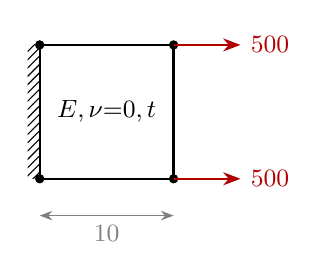
\begin{tikzpicture}[scale=0.85]
  \wall{0}{0}{2}
  \draw[elem] (0,0) rectangle (2,2);
  \foreach \y in {0,2} \node[fnode] at (0,\y) {};
  \foreach \y in {0,2} \node[fnode] at (2,\y) {};
  \draw[load] (2,0) -- (3,0) node[right] {\small 500};
  \draw[load] (2,2) -- (3,2) node[right] {\small 500};
  \node at (1,1) {\small $E,\nu{=}0,t$};
  \draw[dim] (0,-0.55) -- (2,-0.55) node[midway,below] {\small $10$};
\end{tikzpicture}
\caption{E1: single Quad4, clamped edge, uniform end load. $\sigma_x=1000$ psi exact.}
\end{figure}

\subsection{E2 --- Quad4 plate far-field stress (mesh-level sanity)}
\textbf{Test:} \texttt{Plate\_20x20\_FarFieldStress}\\
\textbf{Basis:} $100\times100$ plate, $20\times20$ Quad4 mesh, $\nu=0.3$,
one edge clamped, uniform load on the far edge. By Saint-Venant, mid-plate
$\sigma_x = 2100/(100\cdot 0.1) = 210$ psi.\\
\textbf{Acceptance:} mid-plate element average within 2\%.

\begin{figure}[H]\centering
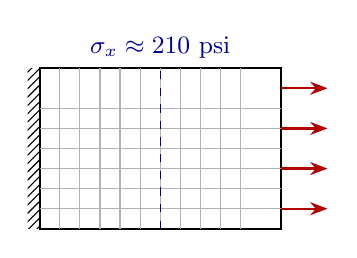
\begin{tikzpicture}[scale=0.85]
  \wall{0}{0}{2.4}
  \draw[elem] (0,0) rectangle (3.6,2.4);
  \foreach \x in {0.3,0.6,...,3.3} \draw[mesh] (\x,0) -- (\x,2.4);
  \foreach \y in {0.3,0.6,...,2.1} \draw[mesh] (0,\y) -- (3.6,\y);
  \foreach \y in {0.2,0.8,1.4,2.0} \draw[load] (3.6,\y+0.1) -- (4.3,\y+0.1);
  \draw[dashed,blue!60!black] (1.8,0) -- (1.8,2.4) node[above] {\small $\sigma_x \approx 210$ psi};
\end{tikzpicture}
\caption{E2: clamped plate under end tension; far-field stress checked at mid-plate.}
\end{figure}

\subsection{E3 --- Quad4 constant-stress patch state through nodal averaging}
\textbf{Test:} \texttt{NodalStresses\_UniformField\_EqualElementStress}\\
\textbf{Basis:} $2\times2$ mesh with \emph{consistent} edge loads (corner
nodes carry half the mid-node value: $250/500/250$ for 1000 total). A
constant stress field must be reproduced exactly at every corner-extrapolated,
node-averaged evaluation point.\\
\textbf{Acceptance:} $\sigma_x=1000$, $\sigma_y=0$, $\sigma_{VM}=1000$ at all
nine averaged nodes (4 decimals); contributing-element counts verified
(interior node 4, edge 2, corner 1).

\begin{figure}[H]\centering
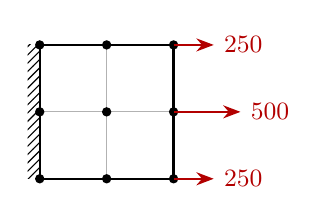
\begin{tikzpicture}[scale=0.85]
  \wall{0}{0}{2}
  \draw[elem] (0,0) rectangle (2,2);
  \draw[mesh] (1,0) -- (1,2); \draw[mesh] (0,1) -- (2,1);
  \foreach \x in {0,1,2} \foreach \y in {0,1,2} \node[fnode] at (\x,\y) {};
  \draw[load] (2,0) -- (2.6,0) node[right] {\small 250};
  \draw[load] (2,1) -- (3.0,1) node[right] {\small 500};
  \draw[load] (2,2) -- (2.6,2) node[right] {\small 250};
\end{tikzpicture}
\caption{E3: consistent loads for uniform traction; averaging must not disturb a constant field.}
\end{figure}

\subsection{E4 --- Quad8 uniaxial patch test}
\textbf{Test:} \texttt{Quad8\_PatchTest\_UniaxialTensionExact}\\
\textbf{Basis:} single 8-node serendipity element. Consistent nodal loads for
uniform traction on a quadratic edge are $\tfrac16 : \tfrac46 : \tfrac16$ of
the edge total. Same closed form as E1.\\
\textbf{Acceptance:} $u=10^{-3}$ at all free-edge nodes (9 decimals);
$\sigma_x$ exact at the centre and at \emph{all eight} averaged node positions
(4 decimals); reaction sum exact.

\begin{figure}[H]\centering
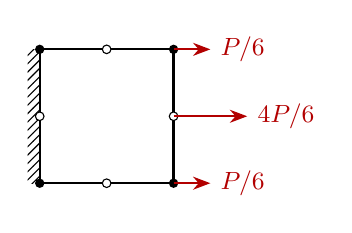
\begin{tikzpicture}[scale=0.85]
  \wall{0}{0}{2}
  \draw[elem] (0,0) rectangle (2,2);
  \foreach \x/\y in {0/0,2/0,2/2,0/2} \node[fnode] at (\x,\y) {};
  \foreach \x/\y in {1/0,2/1,1/2,0/1} \node[mnode] at (\x,\y) {};
  \draw[load] (2,0) -- (2.55,0) node[right] {\small $P/6$};
  \draw[load] (2,1) -- (3.1,1) node[right] {\small $4P/6$};
  \draw[load] (2,2) -- (2.55,2) node[right] {\small $P/6$};
\end{tikzpicture}
\caption{E4: Quad8 patch test (open circles are midside nodes) with consistent quadratic-edge loads.}
\end{figure}

\subsection{E5 --- Quad8 pure in-plane bending (exact linear stress)}
\textbf{Test:} \texttt{Quad8\_PureBending\_ExactLinearStress}\\
\textbf{Basis:} a \emph{single} Quad8 ($20\times10$, mid-plane at $y=0$) under
pure bending applied as a consistent linear end traction
$\sigma_x(y) = 200\,y$. The quadratic displacement field carries linear strain
exactly --- the defining capability a Quad4 lacks (shear locking).\\
\textbf{Acceptance:} $\sigma_x = 200\,y$ reproduced at every node (3 decimals).

\begin{figure}[H]\centering
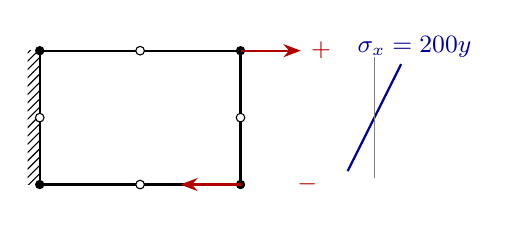
\begin{tikzpicture}[scale=0.85]
  \wall{0}{-1}{1}
  \draw[elem] (0,-1) rectangle (3,1);
  \foreach \x/\y in {0/-1,3/-1,3/1,0/1} \node[fnode] at (\x,\y) {};
  \foreach \x/\y in {1.5/-1,3/0,1.5/1,0/0} \node[mnode] at (\x,\y) {};
  \draw[load] (3,1) -- (3.9,1) node[right] {\small $+$};
  \draw[load] (3,-1) -- (2.1,-1); \node[red!70!black] at (4.0,-1) {\small $-$};
  \draw[blue!60!black,thick] (4.6,-0.8) -- (5.4,0.8);
  \draw[gray] (5.0,-0.9) -- (5.0,0.9);
  \node[blue!60!black] at (5.6,1.05) {\small $\sigma_x=200y$};
\end{tikzpicture}
\caption{E5: single Quad8 in pure bending; the recovered stress profile is exactly linear.}
\end{figure}

\subsection{E6 --- Quad8 quarter-point (Barsoum crack-tip) configuration}
\textbf{Test:} \texttt{Quad8\_QuarterPoint\_CrackTipConfigurationSolves}\\
\textbf{Basis:} the two midside nodes adjacent to a ``crack-tip'' corner are
moved to the quarter points. With the fully isoparametric formulation, the
geometry mapping then embeds the $1/\sqrt{r}$ strain singularity used for
stress-intensity-factor extraction. Gauss points are interior, so assembly
remains well-defined; the singularity sits exactly at the tip node.\\
\textbf{Acceptance:} assembles ($\det J > 0$ at all Gauss points), solves, all
displacements and averaged stresses finite, $\Sigma R_y$ balances the applied
load to 5 decimals.

\begin{figure}[H]\centering
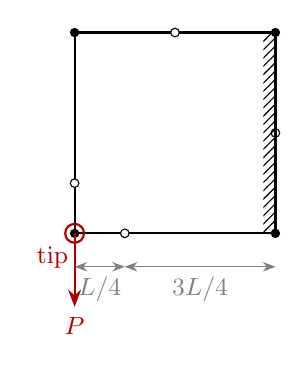
\begin{tikzpicture}[scale=0.85]
  \draw[elem] (0,0) rectangle (3,3);
  \foreach \x/\y in {0/0,3/0,3/3,0/3} \node[fnode] at (\x,\y) {};
  % quarter-point midsides near the tip (corner at origin)
  \node[mnode] at (0.75,0) {}; \node[mnode] at (0,0.75) {};
  \node[mnode] at (3,1.5) {}; \node[mnode] at (1.5,3) {};
  \node[circle,draw=red!70!black,thick,inner sep=2.4pt] at (0,0) {};
  \node[red!70!black,below left] at (0.05,-0.06) {\small tip};
  \draw[dim] (0,-0.5) -- (0.75,-0.5) node[midway,below] {\small $L/4$};
  \draw[dim] (0.75,-0.5) -- (3,-0.5) node[midway,below] {\small $3L/4$};
  \draw[load] (0,0) -- (0,-1.1) node[below] {\small $P$};
  \wall{3}{0}{3}
\end{tikzpicture}
\caption{E6: midside nodes shifted to the quarter points adjacent to the tip corner.}
\end{figure}

\subsection{E7 --- Bar axial stiffness ($\delta = PL/EA$)}
\textbf{Test:} \texttt{Bar\_AxialElongation\_PLOverEA}\\
\textbf{Basis:} $E=10^7$, $A=0.1$, $L=10$, $P=1000 \Rightarrow \delta = 0.01$.
A second, orthogonal bar provides transverse restraint and must carry
$\approx 0$ force.\\
\textbf{Acceptance:} $\delta$ exact to $10^{-9}$; $P=+1000$ (tension-positive),
$\sigma = 10{,}000$ psi; transverse bar force $\le 10^{-6}$.

\begin{figure}[H]\centering
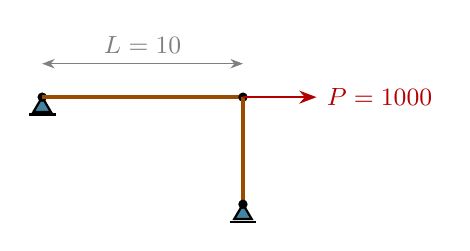
\begin{tikzpicture}[scale=0.85]
  \pin{0}{0}
  \node[fnode] at (0,0) {};
  \draw[very thick,orange!60!black] (0,0) -- (3,0);
  \node[fnode] at (3,0) {};
  \draw[very thick,orange!60!black] (3,0) -- (3,-1.6);
  \pin{3}{-1.6}
  \node[fnode] at (3,-1.6) {};
  \draw[load] (3,0) -- (4.1,0) node[right] {\small $P=1000$};
  \draw[dim] (0,0.5) -- (3,0.5) node[midway,above] {\small $L=10$};
\end{tikzpicture}
\caption{E7: axial bar with transverse support bar; elongation and force sign verified.}
\end{figure}

\subsection{E8 --- Spring element (XY-decoupled fastener idealisation)}
\textbf{Test:} \texttt{Spring\_DecoupledXY\_ForceAndDisplacement}\\
\textbf{Basis:} the spring applies independent stiffness $k$ in X and Y (it is
deliberately \emph{not} axial --- this is the sheet load-transfer fastener
idealisation). $F = k\delta$: $k=10^5$, $F=100 \Rightarrow \delta = 10^{-3}$.\\
\textbf{Acceptance:} $\delta$ and the recovered spring force exact to $10^{-9}$.

\begin{figure}[H]\centering
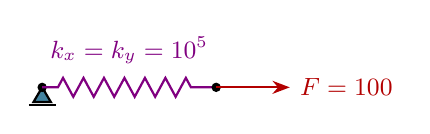
\begin{tikzpicture}[scale=0.85]
  \pin{0}{0}
  \node[fnode] at (0,0) {};
  \draw[spring] (0,0) -- (2.6,0);
  \node[fnode] at (2.6,0) {};
  \draw[load] (2.6,0) -- (3.7,0) node[right] {\small $F=100$};
  \node[violet] at (1.3,0.55) {\small $k_x = k_y = 10^5$};
\end{tikzpicture}
\caption{E8: decoupled spring; force--displacement relation exact per direction.}
\end{figure}

% =====================================================================
\section{Boundary conditions and constraints}
% =====================================================================

\subsection{C1 --- Enforced displacement is exact (direct elimination)}
\textbf{Test:} \texttt{EnforcedDisplacement\_IsExact}\\
\textbf{Basis:} prescribed $d_x = 2\times10^{-3}$ on the free edge of the E1
plate $\Rightarrow \sigma_x = E\varepsilon = 2000$ psi. Prescribed values are
applied by direct elimination (partitioned solve), so there is \emph{no}
penalty-number approximation.\\
\textbf{Acceptance:} prescribed displacement reproduced to 12 decimals;
$\sigma_x$ to $10^{-3}$.

\begin{figure}[H]\centering
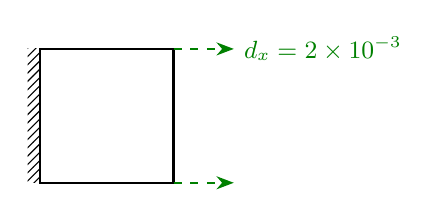
\begin{tikzpicture}[scale=0.85]
  \wall{0}{0}{2}
  \draw[elem] (0,0) rectangle (2,2);
  \draw[enf] (2,0) -- (2.9,0);
  \draw[enf] (2,2) -- (2.9,2) node[right] {\small $d_x = 2\times10^{-3}$};
\end{tikzpicture}
\caption{C1: enforced edge displacement (dashed green); stress matches $E\varepsilon$ exactly.}
\end{figure}

\subsection{C2 --- RBE2 ties selected DOFs exactly}
\textbf{Test:} \texttt{Rbe2\_TiesSelectedDofsExactly}\\
\textbf{Basis:} RBE2 is enforced as an \emph{exact multipoint constraint}: tied
DOFs share one solve unknown (no penalty). Here the loaded edge of a plate is
tied in X only, with the load applied to a single node of the group.\\
\textbf{Acceptance:} all tied $d_x$ identical to 12 decimals; $d_y$
demonstrably independent (Poisson contraction differs); the reaction sum
carries the full load through the tie.

\begin{figure}[H]\centering
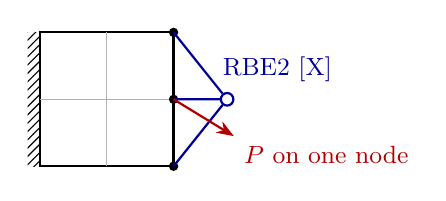
\begin{tikzpicture}[scale=0.85]
  \wall{0}{0}{2}
  \draw[elem] (0,0) rectangle (2,2);
  \draw[mesh] (1,0) -- (1,2); \draw[mesh] (0,1) -- (2,1);
  \foreach \y in {0,1,2} \node[fnode] at (2,\y) {};
  % spider
  \node[rbe,circle,draw,inner sep=1.6pt] (ind) at (2.8,1) {};
  \draw[rbe] (ind) -- (2,0); \draw[rbe] (ind) -- (2,1); \draw[rbe] (ind) -- (2,2);
  \node[rbe] at (3.55,1.45) {\small RBE2 [X]};
  \draw[load] (2,1) -- (2.9,0.45) node[below right] {\small $P$ on one node};
\end{tikzpicture}
\caption{C2: edge tied in X by an RBE2 spider; load on one node moves the whole group.}
\end{figure}

\subsection{C3 --- Constraint applied through the independent node}
\textbf{Test:} \texttt{Rbe2\_ConstrainsViaIndependentNode}\\
\textbf{Basis:} a BC anywhere in a tie group holds the group, and loads on
dependent nodes act on the group. A bar (PL/EA) carries the tied pair; the
closed form must be recovered.\\
\textbf{Acceptance:} group displacements identical (12 decimals);
$\delta = PL/EA$ to 9 decimals; reaction sum exact.

\subsection{C4 --- Conflicting prescribed values inside a tie group}
\textbf{Test:} \texttt{Rbe2\_ConflictingPrescribedValues\_Throw}\\
\textbf{Basis:} two different enforced displacements within one tie group are
physically contradictory.\\
\textbf{Acceptance:} a clear solver error --- never a silently averaged or
garbage answer.

\begin{figure}[H]\centering
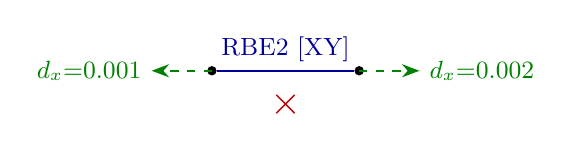
\begin{tikzpicture}[scale=0.85]
  \node[fnode] (a) at (0,0) {}; \node[fnode] (b) at (2.2,0) {};
  \draw[rbe] (a) -- (b); \node[rbe] at (1.1,0.32) {\small RBE2 [XY]};
  \draw[enf] (0,0) -- (-0.9,0) node[left] {\small $d_x{=}0.001$};
  \draw[enf] (2.2,0) -- (3.1,0) node[right] {\small $d_x{=}0.002$};
  \node[red!70!black] at (1.1,-0.5) {\Large $\times$};
\end{tikzpicture}
\caption{C4: contradictory enforced values in one rigid group are rejected.}
\end{figure}

% =====================================================================
\section{Solution diagnostics (error-trapping verification)}
% =====================================================================

\subsection{D1 --- Orphan node diagnostic}
\textbf{Test:} \texttt{OrphanNode\_ThrowsWithNodeId}\\
\textbf{Basis:} a node with no attached stiffness makes $K$ singular; a
pre-solve check names the offending node(s) instead of failing opaquely.\\
\textbf{Acceptance:} the error message contains the orphan node id.

\subsection{D2 --- Under-constrained model detection (residual guard)}
\textbf{Test:} \texttt{UnderConstrained\_ThrowsInsteadOfSilentGarbage}\\
\textbf{Basis:} with rigid-body modes present, the sparse LU factorisation does
\emph{not} necessarily throw --- it can return zeros. Every solution is
therefore checked against $\lVert K u - f \rVert \le 10^{-6}\,\lVert f \rVert$.\\
\textbf{Acceptance:} a loaded but unconstrained plate raises a clear
``add constraints'' error.

\begin{figure}[H]\centering
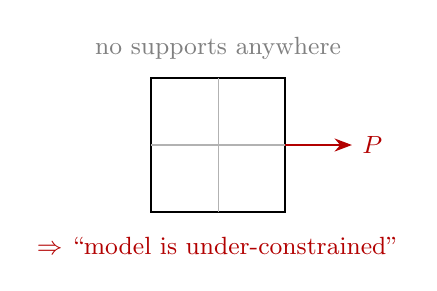
\begin{tikzpicture}[scale=0.85]
  \draw[elem] (0,0) rectangle (2,2);
  \draw[mesh] (1,0) -- (1,2); \draw[mesh] (0,1) -- (2,1);
  \draw[load] (2,1) -- (3,1) node[right] {\small $P$};
  \node[gray] at (1,2.45) {\small no supports anywhere};
  \node[red!70!black] at (1,-0.5) {\small $\Rightarrow$ ``model is under-constrained''};
\end{tikzpicture}
\caption{D2: rigid-body modes are caught by the post-solve equilibrium residual check.}
\end{figure}

% =====================================================================
\section{Stress recovery (nodal averaging)}
% =====================================================================

\subsection{S1 --- Constant field invariant under averaging}
\textbf{Test:} \texttt{NodalStresses\_UniformField\_EqualElementStress}
(shared with E3). A constant stress state must survive corner extrapolation
and node averaging unchanged at every node.

\subsection{S2 --- Step change averages to the mean at shared nodes}
\textbf{Test:} \texttt{NodalStresses\_StepChange\_AveragesAtSharedNodes}\\
\textbf{Basis:} two elements in series with different thickness override:
$\sigma_x = P/(t\,w)$ gives 500 psi in the thick element and 1000 psi in the
thin one. At the shared interface nodes the average of the two corner values,
750 psi, must be reported.\\
\textbf{Acceptance:} per-node values 500 / 750 / 1000 to 3 decimals.

\begin{figure}[H]\centering
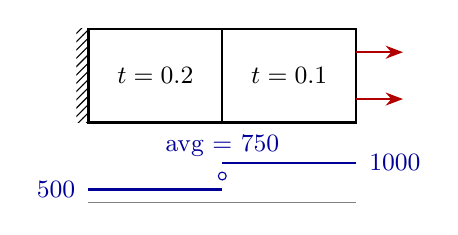
\begin{tikzpicture}[scale=0.85]
  \wall{0}{0}{1.4}
  \draw[elem] (0,0) rectangle (2,1.4);
  \draw[elem] (2,0) rectangle (4,1.4);
  \node at (1,0.7) {\small $t=0.2$}; \node at (3,0.7) {\small $t=0.1$};
  \draw[load] (4,0.35) -- (4.7,0.35); \draw[load] (4,1.05) -- (4.7,1.05);
  % stress profile
  \draw[gray] (0,-1.2) -- (4,-1.2);
  \draw[blue!60!black,thick] (0,-1.0) -- (2,-1.0);
  \draw[blue!60!black,thick] (2,-0.6) -- (4,-0.6);
  \node[fill=white,circle,draw=blue!60!black,inner sep=1pt] at (2,-0.8) {};
  \node[blue!60!black,right] at (4.05,-0.6) {\small 1000};
  \node[blue!60!black,left] at (-0.05,-1.0) {\small 500};
  \node[blue!60!black] at (2,-0.35) {\small avg = 750};
\end{tikzpicture}
\caption{S2: thickness step; the averaged nodal value at the interface is the exact mean.}
\end{figure}

% =====================================================================
\section{Model-operation verification}
% =====================================================================

These cases verify that meshing and editing operations always leave a valid,
solvable model: element references intact, ids unique, no dangling entities.
Cases with significant physical content are sketched.

\begin{table}[H]\small\centering
\begin{tabular}{@{}llp{8.6cm}@{}}
\toprule
ID & Test & What it proves \\
\midrule
M1 & \texttt{Mesher\_FlatQuad\_NodeAndElementCounts} & Structured-mesh counts; corner FE nodes coincide with geometry; re-mesh \emph{fully replaces} the old mesh (unique ids, valid references); result solves \\
M2 & \texttt{Mesher\_ArcEdge\_MatchesWebtoolSample} & Circular-arc edge geometry matches the webtool mesher to 4 decimals (cross-implementation consistency) \\
M3 & \texttt{Quad8\_Mesher\_CountsAndMidsides} & Serendipity grid count $(2M{+}1)(2N{+}1)-MN$; midsides exactly at edge midpoints; Quad4$\leftrightarrow$Quad8 re-mesh switches cleanly \\
M4 & \texttt{Mesher\_MoveGeometryPoint\_RemeshesAffectedSurfaces} & Geometry edits re-mesh affected surfaces with stored divisions; mesh follows geometry; unmeshed surfaces untouched \\
M5 & \texttt{Mesher\_DeleteElements\_RemovesOrphanNodes} & Element deletion removes newly unreferenced nodes \\
M6 & \texttt{Mesher\_DeleteNodes\_CascadesToAttachedEntities} & Node deletion cascades to elements/springs/bars/RBE2s; remaining references intact \\
M7 & \texttt{Mesher\_DeleteSurface\_RemovesMeshAndOrphanGeometry} & Surface deletion removes its mesh, attached entities, unshared geometry points \\
M8 & \texttt{Mesher\_ClearMesh\_KeepsNodesSharedWithOtherSurfaces} & After stitching, clearing one surface keeps seam nodes the other still references \\
M11 & \texttt{Mesher\_MergeCoincidentNodes\_NegativeCoordinates} & Coincidence search correct for negative / origin-straddling coordinates \\
M12 & \texttt{Mesher\_AddSurface\_SharedPoints} & Snapped corner picks share geometry points; moving a shared point re-meshes both surfaces; duplicate corners rejected \\
M13 & \texttt{Mesher\_SpringPointGrid\_CountsAndSpacing} & Grid counts, pitch, collapsed single-row/column behaviour \\
M16 & \texttt{Rbe2\_CleanupOnMeshAndMergeOperations} & RBE2s pruned on re-mesh; references remapped through merges \\
\bottomrule
\end{tabular}
\caption{Model-operation integrity cases (tabulated).}
\end{table}

\subsection{M9 --- Coincident-node merge stitches two meshes into one plate}
\textbf{Test:} \texttt{Mesher\_MergeCoincidentNodes\_StitchesTwoSurfacesIntoContinuousPlate}\\
\textbf{Basis:} two $5\times10$ surfaces meshed separately share the $x=5$
line as duplicated seam nodes. After merging, the pair must behave as one
continuous $10\times10$ plate: uniaxial tension gives the exact bilinear
answer.\\
\textbf{Acceptance:} 3 seam nodes merged; every element keeps valid node
references; $\sigma_x = 1000$ psi in \emph{every} element (4 decimals);
reactions balance.

\begin{figure}[H]\centering
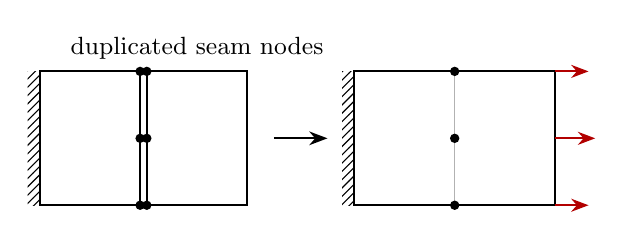
\begin{tikzpicture}[scale=0.85]
  \wall{0}{0}{2}
  \draw[elem] (0,0) rectangle (1.5,2);
  \draw[elem] (1.6,0) rectangle (3.1,2);
  \foreach \y in {0,1,2} {\node[fnode] at (1.5,\y) {}; \node[fnode] at (1.6,\y) {};}
  \node at (2.35,2.35) {\small duplicated seam nodes};
  \draw[-{Stealth},thick] (3.5,1) -- (4.3,1);
  \begin{scope}[shift={(4.7,0)}]
    \wall{0}{0}{2}
    \draw[elem] (0,0) rectangle (3,2);
    \draw[mesh] (1.5,0) -- (1.5,2);
    \foreach \y in {0,1,2} \node[fnode] at (1.5,\y) {};
    \draw[load] (3,0) -- (3.5,0); \draw[load] (3,1) -- (3.6,1); \draw[load] (3,2) -- (3.5,2);
  \end{scope}
\end{tikzpicture}
\caption{M9: merge within tolerance fuses the seam; the stitched pair recovers the exact one-plate answer.}
\end{figure}

\subsection{M10 --- Merge never destroys spring-joined fastener pairs}
\textbf{Test:} \texttt{Mesher\_MergeCoincidentNodes\_PreservesSpringPairsAndBcs}\\
\textbf{Basis:} coincident nodes joined by a spring are the intentional
fastener idealisation; merging them would silently delete the modelled load
transfer. Plain coincident pairs do merge; BCs carry to the surviving node;
zero-length bars created by a merge are removed; a selection-scoped merge
leaves out-of-scope nodes untouched.

\begin{figure}[H]\centering
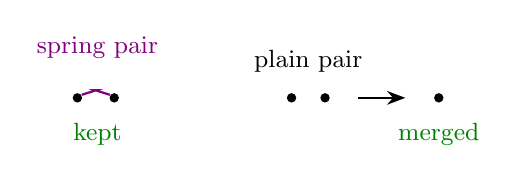
\begin{tikzpicture}[scale=0.85]
  \node[fnode] (a) at (0,0) {}; \node[fnode] (b) at (0.55,0) {};
  \draw[spring] (a) to[bend left=35] (b);
  \node[violet] at (0.3,0.75) {\small spring pair};
  \node[green!50!black] at (0.3,-0.55) {\small kept};
  \node[fnode] (c) at (3.2,0) {}; \node[fnode] (d) at (3.7,0) {};
  \node at (3.45,0.55) {\small plain pair};
  \draw[-{Stealth},thick] (4.2,0) -- (4.9,0);
  \node[fnode] at (5.4,0) {};
  \node[green!50!black] at (5.4,-0.55) {\small merged};
\end{tikzpicture}
\caption{M10: spring-connected coincident pairs are exempt from merging.}
\end{figure}

\subsection{M14/M15 --- Springs at spring points: exactly-two rule and visibility scope}
\textbf{Tests:} \texttt{Mesher\_SpringsAtSpringPoints\_ExactlyTwoVisibleNodesRule},
\texttt{Mesher\_SpringsAtSpringPoints\_OnlyVisibleNodesConsidered}\\
\textbf{Basis:} at each spring point, a spring is created only when
\emph{exactly two visible} FE nodes lie within the coincidence range (one
spring per point; duplicates skipped; $>2$ in range is skipped, not guessed).
With three coincident layers nothing is created until one layer is hidden ---
then the remaining pair connects, and no spring touches the hidden layer.

\begin{figure}[H]\centering
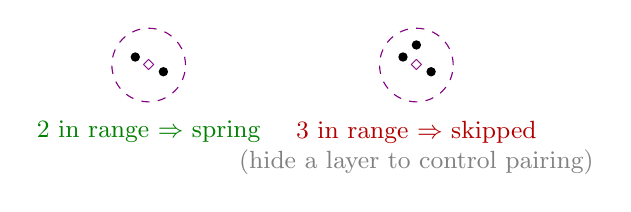
\begin{tikzpicture}[scale=0.85]
  % left: ok case
  \draw[violet,dashed] (0,0) circle (0.55);
  \node[violet] (sp) at (0,0) {\footnotesize$\diamond$};
  \node[fnode] at (-0.2,0.12) {}; \node[fnode] at (0.22,-0.1) {};
  \node[green!50!black] at (0,-1.0) {\small 2 in range $\Rightarrow$ spring};
  % right: too many
  \begin{scope}[shift={(4,0)}]
    \draw[violet,dashed] (0,0) circle (0.55);
    \node[violet] at (0,0) {\footnotesize$\diamond$};
    \node[fnode] at (-0.2,0.12) {}; \node[fnode] at (0.22,-0.1) {}; \node[fnode] at (0.0,0.3) {};
    \node[red!70!black] at (0,-1.0) {\small 3 in range $\Rightarrow$ skipped};
    \node[gray] at (0,-1.45) {\small (hide a layer to control pairing)};
  \end{scope}
\end{tikzpicture}
\caption{M14/M15: the exactly-two-visible-nodes rule for automatic fastener creation.}
\end{figure}

% =====================================================================
\section{System level and file integrity}
% =====================================================================

\begin{table}[H]\small\centering
\begin{tabular}{@{}llp{8.6cm}@{}}
\toprule
ID & Test & What it proves \\
\midrule
F1 & \texttt{SampleModel\_LoadsAndSolves} & A real webtool-exported model (curved edge, BCs, bars) loads, solves, satisfies equilibrium ($\Sigma R_x$ to 4 decimals), all displacements finite and bounded \\
F2 & \texttt{WebtoolJson\_RoundTrip} & Webtool JSON compatibility: camelCase fields, edge radii, BCs, springs, bars survive load $\to$ save $\to$ load \\
\bottomrule
\end{tabular}
\caption{System-level cases.}
\end{table}

\section{Independent cross-checks performed during development}

Not part of the automated suite, recorded for completeness:
\begin{itemize}
  \item The webtool's solver (the same element formulation, independently
        implemented in JavaScript) passes the equivalents of E1, E7, E8, C1,
        D1 and E2 in its own headless Node.js harness --- two independent
        implementations agreeing on the same closed-form answers.
  \item The native and webtool meshers produce numerically identical meshes
        for the same curved-edge model (M2 pins this permanently).
\end{itemize}

\section{Known gaps --- recommended additions for a formal validation suite}

Verification above is largely on rectangular, undistorted elements with
closed-form targets. A formal validation suite should add:

\begin{enumerate}
  \item \textbf{Distorted-element patch tests} (Irons): constant-stress patch
        on irregular Q4/Q8 assemblies. The isoparametric formulation should
        pass; it is currently untested in distorted form.
  \item \textbf{Convergence vs handbook solutions}: plate with central
        circular hole ($K_t \to 3.0$ under refinement); Q8 vs Q4 convergence
        rates on the same problem. (Model \texttt{stress-conc-hole.json} in
        this folder is the candidate geometry.)
  \item \textbf{Quarter-point SIF benchmarks} (once extraction lands):
        centre- and edge-cracked plates vs handbook $K_I$
        (Tada; Rooke \& Cartwright), with mesh-refinement sensitivity.
  \item \textbf{$\nu \ne 0$ single-element checks}: biaxial case with Poisson
        coupling (current single-element exactness cases use $\nu = 0$).
  \item \textbf{Shape-sensitivity sweep}: accuracy vs aspect ratio and skew,
        to set modelling guidance.
  \item \textbf{Large-model conditioning}: solve time and residual-check
        headroom at $10^5$+ DOF.
  \item \textbf{Reactions under non-zero enforced displacement} vs closed form.
  \item \textbf{Fastened-doubler load transfer} end-to-end vs an independent
        solution (e.g.\ Nastran or closed-form one-dimensional joint theory).
        (Models \texttt{fastened-doublers*.json} in this folder are the
        candidates.)
\end{enumerate}

\end{document}
